\documentclass{article}
\usepackage{fancyhdr}
\usepackage{lipsum} % For generating placeholder text, you can remove this in your actual document.
\usepackage[a4paper, left=.5in, right=.5in, top=1in, bottom=1in]{geometry} % Customize margins
\usepackage{lastpage} % For total page count
\usepackage{titling} % For customizing the title page
\usepackage{graphicx}

\usepackage{listings}
\usepackage{xcolor}
\usepackage{amsmath} % Required for mathematical equations

% Define header and footer for the cover page
\fancypagestyle{coverpage}{% Create a custom page style for the cover page
	\fancyhf{}% Clear default header and footer
	\renewcommand{\headrulewidth}{0pt}% Remove the header rule
	\fancyfoot[C]{Page \thepage  / \pageref{LastPage}}
}

% Define header and footer
\pagestyle{fancy}
\fancyhf{} % Clear default header and footer
\fancyhead[L]{Temperature Sensor Readout - Proposed Solution}
\fancyhead[R]{Renato da Veiga Torres}
\fancyfoot[C]{Page \thepage  / \pageref{LastPage}}

% Customize the title page
\renewcommand{\maketitle}{
	\thispagestyle{coverpage}% Apply the cover page style
	\begin{titlepage}
		\centering
		\vspace*{2cm}
		\Huge{\textbf{Temperature Sensor Readout}}\\
		\huge{\textbf{Proposed Solution}}\\
		\vspace{1cm}
		\Large{Renato da Veiga Torres}\\
		\large{renatoveigatorres@gmail.com}\\
		\vspace{1cm}
		\today % Include the date or modify as needed
		\vfill
	\end{titlepage}
}

\begin{document}

	% Use \maketitle to create the cover page
	\maketitle
	
	\newpage % Start content on a new page
	
	\section{REQ01 - Analyze measuring circuit}
	
	\begin{figure}[h]
		\centering % Center the image
		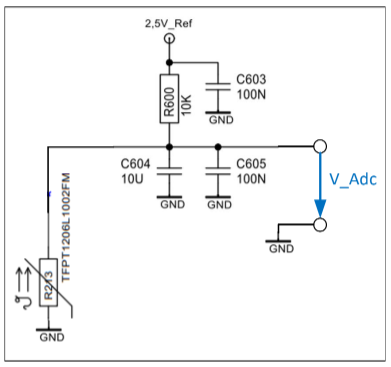
\includegraphics[width=0.5\textwidth]{fig/fig1.png}
		\caption{Temperature measurment circuit}
		\label{fig1}
	\end{figure}
	
	\Large For simplification, ADC input impedance, in this circuit (Figure \ref{fig1}), is considered high enough that is possible to neglect current leaking over ADC pin. In this way, the total current \(i\) on both resistors and \(V_{Adc}\) can be written as in \eqref{eq:eq1}:
		
	\begin{equation}
		\Large i = \frac{V_{Ref}}{R_{600} + R_{213}^{RTC}}
		\label{eq:eq1}
	\end{equation}
	
	As voltage divider, by construction, \(V_{Adc}\) can be calculated as described in \eqref{eq:eq2}:
	
	\begin{equation}
	 	V_{Adc} = \left [\frac{R_{213}^{RTC}}{R_{600} + R_{213}^{RTC}} \right ].V_{Ref}
	 	\label{eq:eq2}
	\end{equation}
	
	
	However, the purpose of the circuit is to 'read' \(V_{Adc}\) value and calculate \(R_{213}^{RTC}\). As \(R_{213}^{RTC}\) is an RTC, its resistance/temperature are unequivocally correlated. Rewriting \eqref{eq:eq2}, \(R_{213}^{RTC}\) value and can be calculated as function of \(V_{Adc}\) as described in \eqref{eq:eq3}:
	
	\begin{equation}
		R_{213}^{RTC} = \left [ \frac{V_{Adc}}{V_{Ref} - V_{Adc}} \right ].R_{600} \label{eq:eq3}
	\end{equation}
	
	As \(R_{600}\) is designed as same TFPT1206L1002FM (in 25° Celsius) - 10 kOhm, the value (\(R_{213}^{RTC}\)/\(R_{600}\)) is same as the \underline{average ratio} (\(R_{Temp}\)/\(R_{25}\)) from datasheet (\underline{tfpt-223737.pdf} - page 3):
	
	\begin{equation}
	ratio = \frac{R_{Temp}}{R_{25}} = \frac{R_{213}^{RTC}}{R_{600}} = \frac{V_{Adc}}{V_{Ref} - V_{Adc}}
	\label{eq:eq4}
	\end{equation}
	
	Obtaining this ratio (\(R_{Temp}\)/\(R_{25}\)) - using \eqref{eq:eq4} is possible to locate (as lookup table) the current temperature of the resistor in the datasheet (\underline{tfpt-223737.pdf} - page 3).
	
	
\section{REQ02 - Implement software that calculates temperature of NTC}
% Define code listing style
\lstdefinestyle{mystyle}{
	language=C,
	backgroundcolor=\color{white},
	basicstyle=\ttfamily\small,
	commentstyle=\color{green!40!black},
	keywordstyle=\color{blue},
	numberstyle=\tiny\color{gray},
	numbers=left,
	numbersep=5pt,
	breaklines=true,
	breakatwhitespace=true,
	tabsize=4,
	captionpos=b,
	frame=single,
}

\lstset{style=mystyle}

	\begin{lstlisting}[caption={C Code for Temperature Sensor}, label=code:temperature_sensor]
		#include "platform_types.h"
		#include "RTC_TFPT1206L1002FM.h"
		
		/**
		* @brief Binary search to find the temperature based on datasheet values.
		*
		* This function performs a binary search on the TFPT_Vishay_Values array to find the
		* temperature corresponding to a target resistance ratio.
		*
		* @param targetRatio The target resistance ratio for which to find the temperature.
		* @return The temperature in degrees Celsius if a match or approximate match is found,
		*         or -273.0f (absolute zero) if the ratio is out of range.
		*/
		static float getTemp_Datasheet(float targetRatio) {
			int low = 0;
			int high = sizeof(TFPT_Vishay_Values) / sizeof(TFPT_Vishay_Values[0]) - 1;
			int resultIndex = -1;
			
			while (low <= high) {
				int mid = low + (high - low) / 2;
				
				if (TFPT_Vishay_Values[mid].fRatio_R25 == targetRatio) {
					resultIndex = mid;
					break;
				}
				
				if (TFPT_Vishay_Values[mid].fRatio_R25 < targetRatio) {
					low = mid + 1;
				} else {
					resultIndex = mid;
					high = mid - 1;
				}
			}
			
			if (resultIndex != -1) {
				// Found the exact match or the next lower fRatio
				if (resultIndex > 0) {
					// Use linearization between 2 datasheet points to optimize accuracy
					// fTx = fT1 + ((fRx - fR1)/(fR2 - fR1))*(T2 - T1);
					// (T2 - T1) is always 1 oC
					float fT1 = TFPT_Vishay_Values[resultIndex - 1].ftemperature;
					float fT2 = TFPT_Vishay_Values[resultIndex].ftemperature;
					float fR1 = TFPT_Vishay_Values[resultIndex - 1].fRatio_R25;
					float fR2 = TFPT_Vishay_Values[resultIndex].fRatio_R25;
					float fTx = fT1 + ((targetRatio - fR1) / (fR2 - fR1));
					return fTx;
				} else {
					return TFPT_Vishay_Values[resultIndex].ftemperature;
				}
			} else {
				// Return 'absolute zero' in case of ratio out of range
				return -273.0f;
			}
		}
		
		/**
		* @brief Calculate the resistance ratio from an ADC value.
		*
		* This function calculates the resistance ratio based on a 12-bit ADC value and
		* the characteristics of the TFPT1206L1002FM sensor.
		*
		* @param uiADCVal The ADC value obtained from the sensor.
		* @return The resistance ratio.
		*/
		static float getRatioFromADCValue(uint16_t uiADCVal) {
			// 12-bit ADC => 2^12 = 4096
			// Range:
			// 0V   - 0
			// 2.5V - 4095
			
			// R213 = [(uiADCVal) / (VREF - uiADCVal)] * R600
			// However, R600 is 10K and R213 (TFPT1206L1002FM) is 10K on 25 oC.
			// R213/R600 = datasheet_ratio itself
			
			uint16_t VREF = 4095;
			float fratio = (uiADCVal) / (VREF - uiADCVal);
			
			return fratio;
		}
		
		/**
		* @brief Get the temperature in degrees Celsius from an ADC value.
		*
		* This function calculates the temperature in degrees Celsius based on the ADC
		* value obtained from the sensor and the datasheet values.
		*
		* @param uiADCVal The ADC value obtained from the sensor.
		* @return The temperature in degrees Celsius if within the valid range,
		*         or -273.0f (absolute zero) if out of range.
		*/
		float getTemperature(uint16_t uiADCVal) {
			return getTemp_Datasheet(getRatioFromADCValue(uiADCVal));
		}
			\end{lstlisting}
	


	
	\section{REQ03 - Implement test-bench for software}
	For this requirement, testbench provided will be used for applying ADC values and confirm/assert Temperatures according implemented code.



	
\end{document}
